\chapter{Αρχιτεκτονική Lambda}
Ένα από τα πιο σύνθετα προβλήματα που χρειάζεται να αντιμετωπίζουν τα Big Data συστήματα είναι η εύρεση λύσης/απάντησης σε πραγματικό χρόνο. Κατά την αρχική τους σχεδίαση, δεν υπήρχε καμία πρόβλεψη για την αντιμετώπιση αυτού του είδους των προβλημάτων και φαινόταν έξω από την σφαίρα των δυνατοτήτων τους. Η υποστήριξη και την ανάπτυξη που έλαβαν τα επόμενα χρόνια, βοήθησαν να αναπτυχθούν και να εδραιωθούν σε όλο και περισσότερους τομείς της πληροφορικής. Ο τομέας των \textit{real-time analytics} αποδείχθηκε ένα αρκετά μεγάλο πρόβλημα, λόγω του όγκου της πληροφορίας που αποθηκεύεται σε ένα τέτοιο σύστημα. Η λύση ακόμα δεν έχει δοθεί από ένα μόνο σύστημα αλλά έχει περιγραφτεί μια αρχιτεκτονική συστημάτων που παράγει το επιθυμητό αποτέλεσμα, με μερικούς περιορισμούς.Η αρχιτεκτονική αυτή ονομάζεται Lambda και οι βασικές της αρχές θα αναλυθούν σε αυτό το κεφάλαιο.

\section{Επίπεδα}
Το αξίωμα της αρχιτεκτονικής Lambda είναι ο χωρισμός του συστήματος σε επίπεδα. Κάθε Big Data σύστημα που την εφαρμόζει θα αποτελεί μια σειρά από επίπεδα, όπου σε κάθε επίπεδο χρησιμοποιείται διαφορετικό σύστημα. Όλα μαζί τα επίπεδα λειτουργούν ως ένα ενιαίο \textit{real-time system}.Το κάθε επίπεδο έχει διαφορετικό σκοπό και ενεργεί σε συνδυασμό με τα αποτελέσματα των επιπέδων κάτω από αυτό. Στην πολύ απλή τους μορφή τα επίπεδα είναι αυτά που φαίνονται στο σχήμα 1.1 .

\begin{figure}[t]
\caption{Επίπεδα της Αρχιτεκτονικής Lambda}
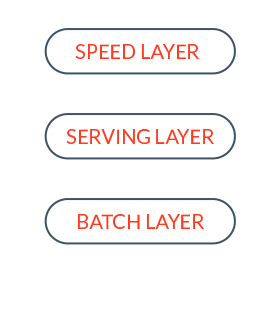
\includegraphics[width=14cm]{images/layers.png}
\centering
\end{figure}
\clearpage

\section{Query}
Ένας πολύ απλός ορισμός των επιπέδων αρκεί, για αυτό το κεφάλαιο, για να γίνει κατανοητή η λειτουργία της Αρχιτεκτονικής Lambda. Το πρόβλημα που πρέπει να λυθεί είναι τα \textit{real-time analytics}. Αυτό μπορεί να συνοψιστεί, για να γίνει πιο γενικό, σε μια πρόταση ως εξής:
\begin{verbatim}
query = function(all data)
\end{verbatim}

Όπου \textit{query} είναι η ερώτηση που υποβάλετε στο σύστημα, η \textit{function} είναι η συνάρτηση υπολογισμού της απάντησης πάνω στα \textit{data}, όλα τα δεδομένα που έχει αποθηκευμένα το σύστημα εκείνη την χρονική στιγμή.
\newline
Στα περισσότερα Big Data συστήματα αυτός ο υπολογισμός θα απαιτούσε από μερικές ώρες μέχρι μερικές ημέρες, δεδομένου του μεγέθους που έχουν τα δεδομένα και την πολυπλοκότητα του υπολογισμού. Για να μπορέσει να απαντηθεί ένα τέτοιο ερώτημα σε \textit{real-time} θα έπρεπε να χρησιμοποιηθούν τεράστιες υποδομές ηλεκτρονικών υπολογιστών και το κόστος, στις περισσότερες περιπτώσεις, για κάτι τέτοιο υπερβαίνει την αξία της απάντησης. Με την Αρχιτεκτονική Lambda αναμένετε η απάντηση να δοθεί σε μερικά δευτερόλεπτα έως λεπτά σε υποδομές πολύ μικρότερης κλίμακας και κόστους. 

\section{Προΰπολογισμός}
Η λύση που υλοποιεί η Αρχιτεκτονική Lambda υποστηρίζετε από τον προϋπολογισμό της απάντησης. Δηλαδή η απάντηση δεν υπολογίζετε από την βασικό dataset την στιγμή που υποβάλετε η ερώτηση, αλλά έχει ήδη υπολογιστεί σε προγενέστερο χρόνο και έχει αποθηκευτεί στο σύστημα. Η προϋπολογισμένη απάντηση, στην Αρχιτεκτονική Lambda, ονομάζετε \textit{batch view}. Πλέον η προηγούμενη μορφή του υπολογισμού έχει πάρει μια διαφορετική μορφή:
\begin{verbatim}
batch view = function (all data)
query = function (batch view)
\end{verbatim}
Τα \textit{batch view} είναι \textit{indexed} για να είναι πιο γρήγορη και εύκολη η εύρεση του σωστού \textit{batch view} και να απαντηθεί το \textit{query} μέσα στον επιθυμητό χρόνο.



\section{Batch Layer}
Το επίπεδο της Αρχιτεκτονικής που υπολογίζει τα \textit{batch view} από το \textit{dataset} ονομάζεται \textit{batch layer} και αποτελεί το πρώτο επίπεδο του συστήματος. Εκτός από τον υπολογισμό των \textit{batch view}, το \textit{batch layer} είναι υπεύθυνο για την αποθήκευση του \textit{master dataset}, δηλαδή των δεδομένων που χρησιμοποιούνται για τον υπολογισμό των \textit{batch view}. Το σύστημα που θα χρησιμοποιηθεί στο \textit{batch layer} θα πρέπει να αποθηκεύει αποδοτικά και με ασφάλεια μεγάλα μεγέθη δεδομένων που συνεχώς θα αυξάνονται, και να εφαρμόζει πάνω τους, τους αλγορίθμους υπολογισμού των \textit{batch view} όποτε εισάγονται νέα δεδομένα στο σύστημα. Τέτοια συστήματα ονομάζονται \textit{batch-processing systems}. Ένα από τα πιο δημοφιλή τέτοια συστήματα είναι το \textbf{Hadoop}, το οποίο θα χρησιμοποιηθεί και σε αυτή την περίπτωση, αλλά θα περιγραφτεί αναλυτικότερα σε επόμενα κεφάλαια.
\newline
Η εισαγωγή δεδομένων στο \textit{batch view} γίνετε με \textit{batch updates}, δηλαδή τα δεδομένα που έρχονται για προσθήκη, δεν εισάγονται αμέσως, αντίθετα αποθηκεύονται προσωρινά σε κάποιο άλλο σύστημα, και μόλις το μέγεθος τους περάσει έναν ορισμένο αριθμό εισάγονται όλα μαζί στο \textit{batch layer}. Αυτή η μέθοδος βοηθάει την απόδοση του συστήματος με δύο τρόπους:
\begin{enumerate}
\item Σε \textit{batch-processing systems}, όπως είναι το \textbf{Hadoop}, των οποίων οι αποθηκευτικές μέθοδοι είναι \textbf{WORM (Write Once Read Many)} η πράξη της εγγραφής είναι ιδιαίτερα δαπανηρή σε υπολογιστική ισχύ και χρόνο. Αυτό συμβαίνει επειδή η πράξη της εγγραφής, για μια ομάδα δεδομένων, θα γίνει μόνο μια φορά στο σύστημα και δεν θα ξαναγίνει. Συνεπώς έχει δοθεί μεγαλύτερη σημασία στην ταχύτητα της ανάγνωσης των δεδομένων, η οποία θα εκτελείτε πολλές φορές. Σε τέτοια συστήματα είναι πιο αποδοτικό να γράφονται πολλά δεδομένα μαζί μια φορά αντί να γίνονται συνεχόμενες εγγραφές, λίγων δεδομένων κάθε φορά.
\item Ο υπολογισμός των νέων \textit{batch view} είναι ιδιαίτερα χρονοβόρος, και το σύστημα καθυστερεί στην εξυπηρέτηση ερωτήσεων όσο υπολογίζει. Συνεπώς η προσθήκη δεδομένων πρέπει να αναβάλετε και να εκτελείτε σε κάποια από τις παρακάτω περιπτώσεις:
\begin{enumerate}
\item Το μέγεθος των νέων δεδομένων έχει περάσει ένα ορισμένο κατώφλι που θεωρείται το σωστό για εισαγωγή στο σύστημα.
\item Είναι μια συγκεκριμένη ώρα/περίοδος της ημέρας που θεωρείται ιδανική για εισαγωγή των νέων δεδομένων λόγω μικρού φόρτου εργασίας και πρόσβασης στο σύστημα εκείνη την ώρα, ακόμα και αν δεν είναι ακόμα στο σωστό μέγεθος.
\end{enumerate}
\end{enumerate}
Μια απεικόνιση του \textit{batch layer} φαίνεται στο σχήμα 1.2.

\begin{figure}[t]
\caption{Batch Layer}
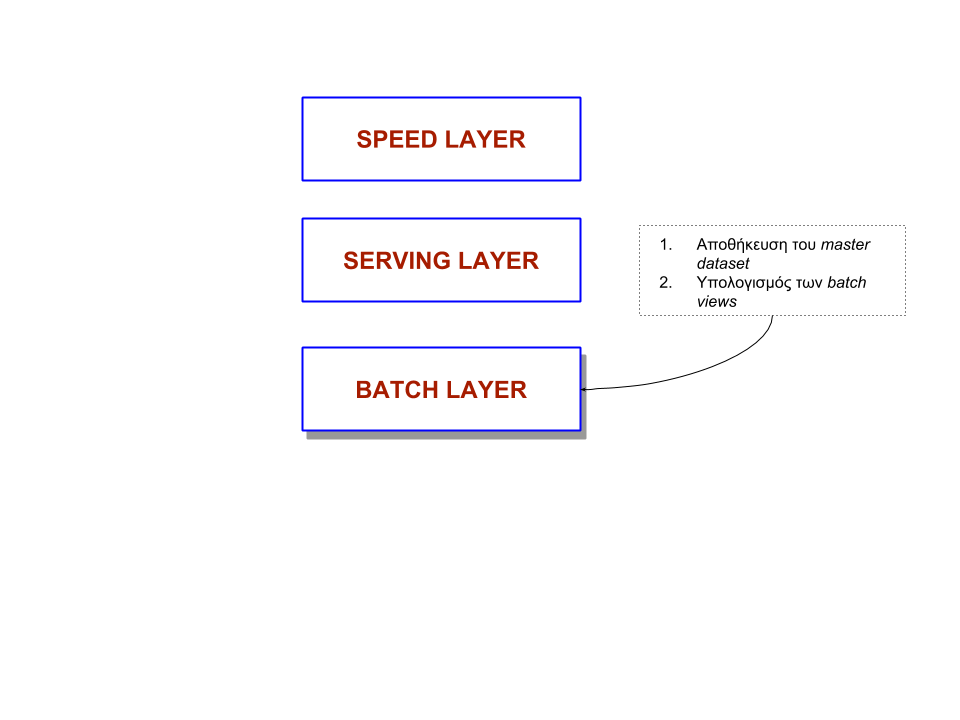
\includegraphics[width=14cm]{images/batch_layer.png}
\centering
\end{figure}
\clearpage

\subsection{Πλεονεκτήματα}
\begin{description}
\item[Παραλληλισμός] Το \textit{batch layer} είναι το πιο απλό και εύκολο στην χρήση επίπεδο της Αρχιτεκτονικής Lambda. Οι αλγόριθμοι που υπολογίζουν τα \textit{batch view} είναι υλοποιημένοι ως γραμμικοί αλγόριθμοι αλλά εκτελούνται παράλληλα χάρη στους μηχανισμούς που προσφέρει το \textit{batch layer}.
\item[Επεκτασιμότητα] Καθώς αυξάνετε ο όγκος των δεδομένων, θα πρέπει να αυξάνετε και το μέγεθος του συστήματος για να αντεπεξέλθει στις απαιτήσεις. Στο \textit{batch layer}, η επέκταση γίνετε απλά με την εισαγωγή νέων μηχανημάτων στο σύστημα.
\item[Ασφάλεια] Η ασφάλεια των δεδομένων που αποθηκεύονται στο \textit{batch layer} διασφαλίζετε με τους μηχανισμούς που προσφέρει το σύστημα, χωρίς να χρειαστεί να σχεδιαστούν πολύπλοκες αρχιτεκτονικές και έλεγχοι από τον διαχειριστή.
\end{description}


\subsection{Μειονεκτήματα}
Το προφανές μειονέκτημα αυτής της υλοποίησης είναι η ανάγκη το σύστημα να γνωρίζει από πριν τις ερωτήσεις που θα του υποβληθούν στο μέλλον. Δεν υπάρχει η δυνατότητα να απαντήσει, σε \textit{real-time}, ερώτηση που δεν έχει καταχωρηθεί στις γνωστές. Επίσης από την στιγμή που θα εισαχθεί μια νέα ερώτηση, υπάρχει ένα χρονικό διάστημα που χρειάζεται για τον υπολογισμό των \textit{batch view} ώστε να είναι σε θέση να την απαντήσει. Αυτό το μειονέκτημα καθιστά την Αρχιτεκτονική Lambda λύση για ένα υποσύνολο των προβλημάτων που ανάγονται σε \textit{real-time analytics} προβλήματα.

\section{Serving Layer}
Το επίπεδο μετά το \textit{batch layer} είναι το \textit{serving layer} το οποίο είναι υπεύθυνο για την αποθήκευση και την χρησιμοποίηση των \textit{batch view} στην απάντηση ερωτήσεων. Στην γενική του μορφή, πρόκειται για μια ειδική \textit{distributed database} η οποία κρατάει το πιο πρόσφατο \textit{batch view}. Κάνοντας \textit{random reads} στο \textit{batch view} απαντάει στα \textit{queries} που υποβάλονται στο σύστημα. Επίσης, μόλις δημιουργηθεί νέο \textit{batch view} είναι υπεύθυνη να αντικαταστήσει το \textit{batch view} που έχει με το καινούργιο ώστε να περιλαμβάνονται και τα νέα δεδομένα στις απαντήσεις.
\newline
Το \textit{serving layer}, συνεπώς, έχει μόνο δύο ενέργειες, τα \textit{random reads} πάνω στο \textit{batch view} που έχει εκείνη την στιγμή, και το \textit{update} του \textit{batch view} κάθε φορά που δημιουργείται καινούργιο. Ένα από τα πιο σύνθετα κομμάτια τέτοιων συστημάτων, \textit{distributed database}, είναι το \textit{random write} που πρέπει να υποστηρίζουν αποδοτικά. Το οποίο, σε αυτή την περίπτωση, δεν χρειάζεται και το σύστημα που χρησιμοποιείται στο  \textit{serving layer} είναι ιδιαίτερα απλό. Σε αυτό το επίπεδο θα χρησιμοποιηθεί η βάση \textbf{ElephantDB} η οποία υποστηρίζει αποδοτικά όλα αυτά που απαιτούνται και είναι πολύ απλή στη χρήση της.
\newline
Μια απεικόνιση του \textit{serving layer} φαίνεται στο σχήμα 1.3.
\begin{figure}[t]
\caption{Serving Layer}
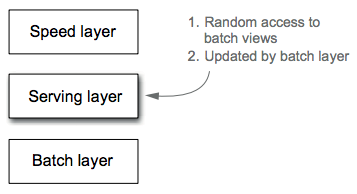
\includegraphics[width=15cm]{images/serving_layer.png}
\centering
\end{figure}
\clearpage


\section{Serving - Batch Layer}
Σε αυτό το σημείο, έχοντας τα δύο επίπεδα \textit{batch} και \textit{serving}, το σύστημα μπορεί να απαντήσει σε \textit{real-time} τις ερωτήσεις που έχουν οριστεί, με μια απόκλιση μερικών ωρών, ανάλογα από το πόσο παλιό είναι το \textit{batch view} που χρησιμοποιείται στο \textit{serving layer}. Επίπλέον, ικανοποιεί όλα τα κριτήρια ενός \textit{Big Data} συστήματος. Αναλυτικότερα:
\begin{description}
\item[Robustness και fault tolerance] Το \textbf{Hadoop} διαχειρίζεται την απενεργοποίηση μηχανημάτων του συστήματος με δικούς του μηχανισμούς σχεδιασμένους να προσφέρουν την μεγαλύτερη δυνατή διαθεσιμότητα. Το \textit{serving layer} χρησιμοποιεί αντίγραφα για το διασφαλίσει και την δικιά του διαθεσιμότητα σε τέτοιες περιπτώσεις.Επιπρόσθετα, και τα δύο επίπεδα είναι ανθεκτικά σε ανθρώπινα λάθη, όπως λάθος δεδομένα ή αλγορίθμους υπολογισμού, επειδή οποιαδήποτε στιγμή τα \textit{batch view} μπορούν να επαναυπολογιστούν με νέους αλγορίθμους και με την διαγραφή των λάθος δεδομένων.
\item [Scalability] Και τα δύο επίπεδα, αποτελούνται από κατανεμημένα συστήματα ειδικά φτιαγμένα ώστε να μπορούν να κάνουν \textit{scale} πολύ εύκολα και γρήγορα.
\item[Generalization] Η αρχιτεκτονική που περιγράφτηκε, ως τώρα, είναι ιδιαίτερα γενική και δεν περιορίζετε στο σύνολο των προβλημάτων που περιγράφονται σε αυτή την περίπτωση μόνο.
\item [Extensibility] Η προσθήκη νέων ερωτήσεων, \textit{views}, αλγορίθμων, δεδομένων είναι πολύ απλή αλλά σε ορισμένες περιπτώσεις απαιτεί κάποιο χρόνο υπολογισμού από το σύστημα.
\item [Ad hoc ερωτήσεις] Από την στιγμή που τα δεδομένα υπάρχουν αποθηκευμένα στο σύστημα, μπορούν να απαντηθούν \textit{ad hoc} ερωτήσεις αλλά δεν θα είναι άμεσα διαθέσιμη η απάντηση, όπως στις προκαθορισμένες ερωτήσεις.
\item [Minimal maintenance] Έχουν επιλεχθεί εύκολα στην εκμάθηση και διατήρηση τους συστήματα για κάθε επίπεδο, για να γίνει η δουλειά του διαχειριστή πιο εύκολη.
\item [Debuggability] Σε κάθε επίπεδο είναι διαθέσιμα τα \textit{inputs} και τα \textit{outputs} των αλγορίθμων, συνεπώς η εύρεση του λάθους γίνετε πιο εύκολη με την σύγκριση των αποτελεσμάτων και των επιθυμητών τιμών.
\end{description}

Με αυτά τα δύο επίπεδα μπορεί να επιλυθεί το πρόβλημα που αναλύθηκε, στην αρχή του κεφαλαίου. Αποτελεί μια απλή και εύκολη σχετικά λύση, χωρίς θέματα συγχρονισμού, και με εύκολη επεκτασιμότητα. Η μόνη λειτουργικότητα που λείπει είναι η άμεση ενημέρωση απαντήσεων με τα καινούργια δεδομένα. Αυτό το εκτελεί το υψηλότερο επίπεδο, το \textit{speed layer}.

\section{Speed Layer}
Κάθε απάντηση που δίνετε, μέχρι στιγμής, από το σύστημα, υπολογίζεται από το νεότερο \textit{batch view} που υπάρχει στο \textit{serving layer}. Τα δεδομένα που φτάνουν στο σύστημα μετά τον υπολογισμό του ενεργού \textit{batch view} και πριν τον υπολογισμό του επόμενου \textit{batch view}, δεν περιλαμβάνονται στις απαντήσεις που δίνονται από το σύστημα σε αυτό το διάστημα. Για να είναι ολοκληρωμένο το σύστημα θα πρέπει να καλυφθεί και αυτή η περίπτωση. Το \textit{speed layer} αναλαμβάνει να υπολογίσει και να βγάλει απαντήσεις από τα πιο πρόσφατα δεδομένα, τα οποία ακόμα δεν έχουν εισαχθεί στο \textit{dataset} του \textit{batch layer}. Όπως φαίνεται από το όνομα του, απαιτείται να είναι πολύ γρήγορο στους υπολογισμούς που θα τρέξει καθώς το σύστημα πρέπει να δώσει την απάντηση σε \textit{real time}.
\newline
Παρομοίως με το \textit{batch layer}, το \textit{speed layer} παράγει \textit{views}, με την διαφορά ότι χρησιμοποιεί μόνο τα πρόσφατα δεδομένα, που δεν έχουν εισαχθεί στο \textit{dataset}. Αυτά τα \textit{views}, ονομάζονται \textit{realtime views}. Επίσης το \textit{speed layer} δεν παράγει συνεχώς καινούργια \textit{views} με κάθε εισαγωγή δεδομένων, αντίθετα ενημερώνει το ήδη υπάρχον \textit{realtime view} ώστε να περιέχει τα καινούργια δεδομένα. Η πράξη του επαναυπολογισμού ολόκληρου του \textit{view} είναι ιδιαίτερα χρονοβόρα όσο περισσότερα δεδομένα μαζεύονται για τους υπολογισμούς, συνεπώς το σύστημα θα χρειάζεται συνεχώς περισσότερο χρόνο για τον υπολογισμό τους.
\newline
Η πράξη που εκτελεί το \textit{speed layer} μπορεί να περιγραφτεί ως εξής:
\begin{verbatim}
realtime view = function(realtime view, new data)
\end{verbatim}
Για την αποθήκευση των νέων δεδομένων και την άμεση πρόσβαση σε αυτά από το \textit{speed layer}, απαιτείται η χρήση μιας βάσης δεδομένων που υποστηρίζει \textit{random reads} και \textit{writes}. Αυτό το κομμάτι, αυξάνει την πολυπλοκότητα και την διαχειριστική δυσκολία του συστήματος.
\newline

Μια απεικόνιση του \textit{speed layer} φαίνεται στο σχήμα 1.4.
\begin{figure}[t]
\caption{Speed Layer}
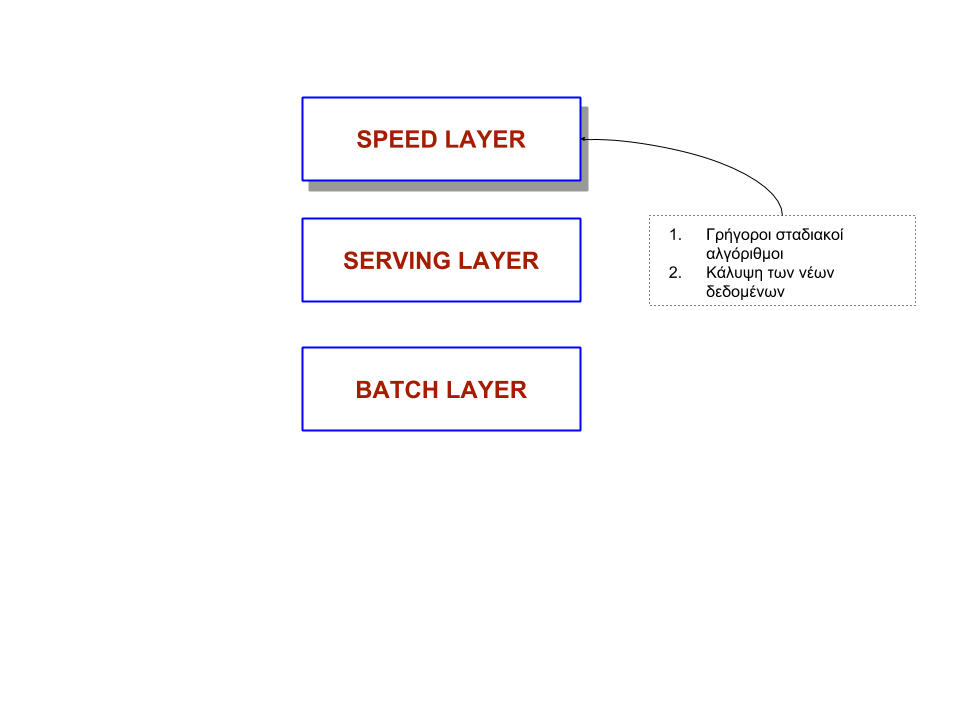
\includegraphics[width=15cm]{images/speed_layer.png}
\centering
\end{figure}
\clearpage

Η τελική απάντηση στην ερώτηση θα βγει ως συνδυασμός του \textit{batch view} και του \textit{realtime view}.

\section{Σύνοψη}
Ανακεφαλαιώνοντας, οι υπολογισμοί της Αρχιτεκτονικής Lambda μπορούν να αποδοθούν ως:
\begin{verbatim}
batch view = function(all data)
realtime view = function(realtime view, new data)
query = function(batch view, realtime view)
\end{verbatim}

Στην εικόνα 1.5 φαίνεται πλέον αναλυτικά ο διαχωρισμός των επιπέδων, και τι περιέχει το καθένα.
\begin{figure}[t]
\caption{Serving Layer}
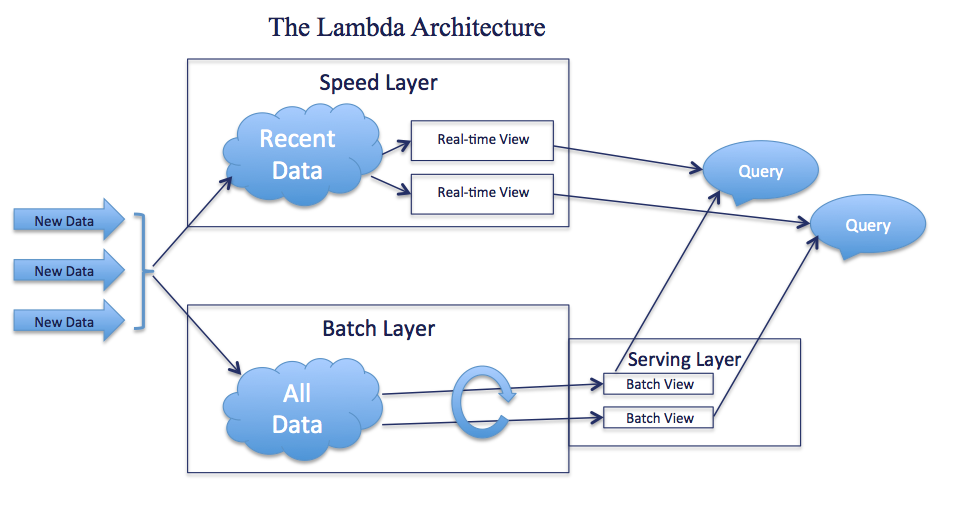
\includegraphics[width=15cm]{images/lambda.png}
\centering
\end{figure}
\clearpage